% !TEX TS-program = xelatex
% !TEX encoding = UTF-8 Unicode
% !Mode:: "TeX:UTF-8"

\documentclass{resume}
\usepackage{graphicx}
\usepackage{tabu}
\usepackage{tabularx}
\usepackage{multirow}
\usepackage{progressbar}
\usepackage{zh_CN-Adobefonts_external} % Simplified Chinese Support using external fonts (./fonts/zh_CN-Adobe/)
\usepackage{tikz}
% \usepackage{NotoSansSC_external}
% \usepackage{NotoSerifCJKsc_external}
% \usepackage{zh_CN-Adobefonts_internal} % Simplified Chinese Support using system fonts
\usepackage{linespacing_fix} % disable extra space before next section
\usepackage{cite}

\newcommand{\hlink}[1]{\href{#1}{#1}}

\begin{document}
\pagenumbering{gobble} % suppress displaying page number

\medskip\noindent
\begin{minipage}{0.7\textwidth}
  \Large{
    \begin{tabu}  { l }
      \scshape{唐宗勋} \\
      \email{tangzongxun@hotmail.com} \\
      \phone{(+86) 13070156080} \\
      \linkedin[tangzongxun]{https://www.linkedin.com/in/tangzongxun} \\
    \end{tabu}
  }
\end{minipage}
\begin{minipage}{0.3\textwidth}
  \raggedleft
  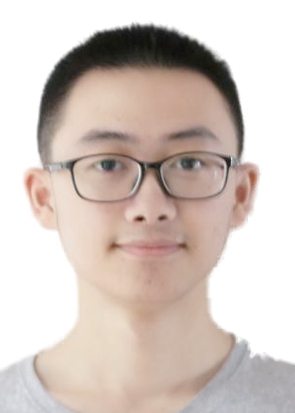
\includegraphics[height=30mm]{me}
\end{minipage}

% \name{唐宗勋}
%
% \basicInfo{
%   \email{tangzongxun@hotmail.com} \textperiodcentered\ 
%   \phone{(+86) 13070156080} \textperiodcentered\ 
%   \linkedin[tangzongxun]{https://www.linkedin.com/in/tangzongxun}}


\section{\faGraduationCap\  教育背景}
\datedsubsection{\textbf{北京航空航天大学}, 北京}{2017 -- 至今}
\textit{在读硕士研究生}\ 电子与通信工程, 预计 2020 年 1 月毕业
\datedsubsection{\textbf{北京航空航天大学}, 北京}{2013 -- 2017}
\textit{学士}\ 电子信息工程

\section{\faUsers\ 实习/项目经历}
\datedsubsection{\textbf{libsm}}{2018年3月 -- 2018年7月}
\role{Rust}{实验室项目,和秘猿科技合作}
主要作者, \hlink{https://github.com/cryptape/libsm}
\begin{itemize}
  \item Rust 语言的中国国家商用密码算法库
  \item 实现了对称加密、哈希函数、数字签名功能
  \item 已经应用于 CITA 项目(\hlink{https://github.com/cryptape/cita})中
\end{itemize}

\datedsubsection{\textbf{pec-client}}{2018年10月 -- 2019年1月}
\role{JavaScript, React}{实验室项目}
\begin{onehalfspacing}
区块链 DApp 前端, \hlink{https://github.com/BH-Open-Blockchain-XLab/pec-client}
\begin{itemize}
  \item 采用 React/Redux 框架的单页应用
  \item 实现了登录、交易显示、交易提交等功能
\end{itemize}
\end{onehalfspacing}

\datedsubsection{\textbf{故事分享机}}{2017年12月 -- 2018年1月}
\role{树莓派, Python}{个人项目}
\begin{onehalfspacing}
负责硬件部分,实现了联网打印功能
\begin{itemize}
  \item 使用了树莓派和热敏打印机
  \item 定期从后台抓取文章,在按动按钮时随机打印
  \item 已经稳定完成了上万份打印任务
\end{itemize}
\end{onehalfspacing}


\section{\faCogs\ IT 技能}
% increase linespacing [parsep=0.5ex]
\begin{itemize}[parsep=0.5ex]
  \item 编程语言: C/C++、Python、JavaScript、Rust
  \item 平台: Linux
  \item 工具: Git、Docker
  \item 领域技能: 密码学、Web 前端、信号处理、嵌入式开发
\end{itemize}

\section{\faHeartO\ 获奖情况}
\datedline{\textit{二等奖}, 全国大学生电子设计竞赛(北京赛区)}{2015 年 8 月}

\section{\faInfo\ 其他}
% increase linespacing [parsep=0.5ex]
\begin{itemize}[parsep=0.5ex]
  \item 语言: 英语 - 熟练(CET-6 546)
\end{itemize}

\end{document}
